\section{Lugar para toma de muestras}

Para la toma de las muestras se eligió un lugar de la ciudad donde el flujo de vehículos es considerablemente constante. Este lugar fue en la calzada las Torres frente a Plaza San Isidro en la ciudad de Culiacán, Sinaloa. Una parte de las muestras fueron tomadas en las mañanas entre las 10 y las 12 A.M. mientras que otra parte de las muestras fueron tomadas entre las 5 y 7 P.M. las muestras nos pueden proporcionar una idea de cuáles son las horas en las que hay un mayor flujo de vehículos, para el caso de este lugar la tarde es cuando hay un flujo vehicular mayor, ya que en algunos casos de las muestras hay hasta 30 segundos con ausencia de vehículos en las muestras tomadas en la mañana. La Figura \ref{fig:LugarMuestras} es del lugar donde se tomaron las muestras.

\begin{figure}[H]
    \centering
    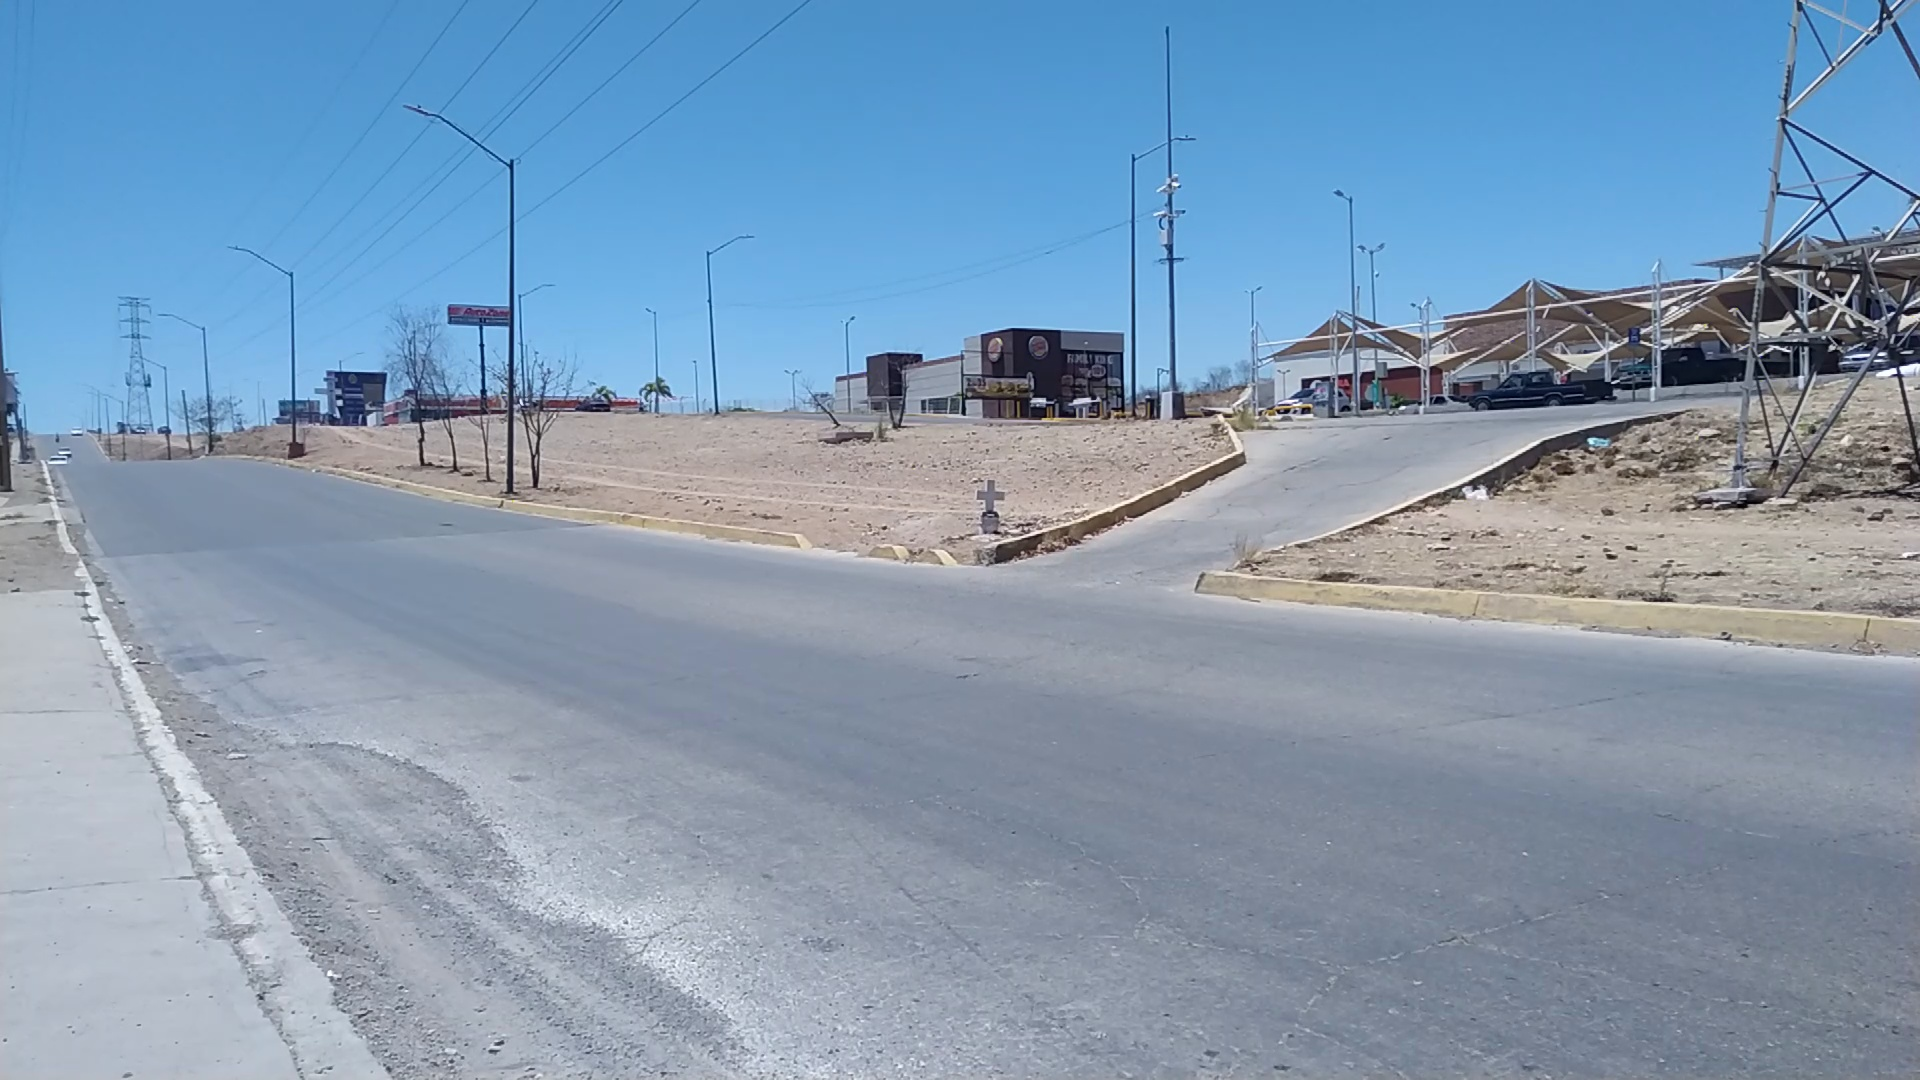
\includegraphics[width=0.9\textwidth]{Resultados/imgs/LugarMuestras.jpg}
    \caption{Lugar donde fueron tomadas las muestras.}
    \label{fig:LugarMuestras}
\end{figure}

Este lugar tiene un flujo de oeste a este, lo cual para la cámara es un flujo de derecha a izquierda. También podemos notar que la calle por la cual pasan los vehículos no está nivelada, para la vista de la cámara los vehículos pasan de arriba hacia abajo. Como se mencionó en la Metodología, hubo especial cuidado a la hora de posicionar la cámara para que los vehículos no pasen paralelamente a la vista de la misma, por lo que se posicionó apuntando un poco hacia la subida de la calle.
